\label{sec:algorithm}

We now use the insight from Sections \ref{sec:prelim} and \ref{sec:il-failure} to construct an update, applied to the expert policy, which improves the expected reward ahead under the implicit policy.  Crucially, this update is designed such that, when interleaved with AIL, the optimal partially observed policy is recovered.  We refer to this iterative algorithm as adaptive asymmetric DAgger (A2D). To derive the update to the expert, $\pi_{\theta}$, we first consider the RL objective under the implicit policy, $\hat{\pi}_{\theta}$:
\begin{align}
     &J(\theta) = \mathop{\mathbb{E}}_{d^{{\hat{\pi}_{\theta}}}(b) \hat{\pi}_\theta(a|b) } \left[ Q^{{\hat{\pi}_{\theta}}}(a,b) \right], \where \\
    & Q^{{\hat{\pi}_{\theta}}}(a,b) =\!\!\!\! \mathop{\mathbb{E}}_{ p(b',s',s|a,b)} \!\bigg[ r(s,a,s') + \!\!\! \mathop{\gamma\mathbb{E}}_{\hat{\pi}_\theta(a'|b')} \! \left[ Q^{\hat{\pi}_\theta} (a', b') \right] \bigg] \!. \nonumber 
\end{align}
This objective defines the cumulative reward of the trainee in terms of the parameters of the expert policy. This means that maximizing $J(\theta)$ maximizes the reward obtained by the implicit policy, and ensures proper expert supervision:
\begin{theorem}[Convergence of Exact A2D]
\label{thm:conv_exact} 
Under exact intermediate updates, the following iteration converges to an optimal partially observed policy $\pi_{\psi^*}(a|b)\in\Pi_{\Psi}$, provided both  $\Pi_{\Phi^*} \subseteq \hat{\Pi}_{\Theta^*} \subseteq \Pi_{\Psi}$:
\begin{align}
    \!&\psi_{k+1} \! = \! \mathop{\argmin}_{\psi \in \Psi} \!\mathop{\mathbb{E}}_{d^{\pi_{\psi_k}}(s,b)} \!\! \left[ \mathbb{KL} \left[ \pi_{\hat{\theta}^*}(a|s) || \pi_\psi(a|b) \right] \right], \label{eq:implicit_ail_argmin}\\
    &\where  \hat{\theta}^* = \mathop{\argmax}_{\theta \in \Theta} \mathop{\mathbb{E}}_{\hat{\pi}_{\theta}(a | b) d^{{\pi_{\psi_k}}}(b)} \left[Q^{{\hat{\pi}_{\theta}}}(a,b) \right]. \label{eq:implicit_rl_argmin}
\end{align}
\end{theorem}
\vspace{-0.2cm}
\begin{proof}
\vspace{-0.2cm}
See Appendix \ref{supp:thoery}.
\end{proof}
\vspace{-0.2cm}
First, an inner optimization, defined by \eqref{eq:implicit_rl_argmin}, maximizes the expected reward of the implicit policy by updating the parameters of the \emph{expert} policy, under the current trainee policy.  The outer optimization, defined by \eqref{eq:implicit_ail_argmin}, then updates the trainee policy by projecting onto the updated implicit policy defined by the updated expert. This projection is performed by minimizing the divergence to the updated expert, as per Theorem \ref{def:ail}.  %\aw{halp}
% This algorithm can be considered as a projected optimization~\cite{bertsekas2014constrained}. 

Unfortunately, directly differentiating through $Q^{\hat{\pi}_\theta}$, or even sampling from $\hat{\pi}_\theta$, is intractable.  We therefore optimize a surrogate reward instead, denoted $J_{\psi}(\theta)$, that defines a lower bound on the objective function in \eqref{eq:implicit_rl_argmin}.  This surrogate is defined as the expected reward ahead under the variational trainee policy $Q^{{\pi_{\psi}}}$.  By maximizing this surrogate objective, we maximize a lower bound on the possible improvement to the implicit policy with respect to the parameters of the expert:
\begin{align}
    \max_{\theta \in \Theta} J_{\psi}(\theta) &= \max_{\theta \in \Theta} \mathop{\mathbb{E}}_{{\hat{\pi}_\theta(a|b) d^{{\pi_{\psi}}}(b)}} \left[ Q^{{\pi_{\psi}}}(a,b) \right] \label{equ:bound:1}\\
    \leq \max_{\theta \in \Theta} J(\theta) &= \max_{\theta \in \Theta}  \mathop{\mathbb{E}}_{{\hat{\pi}_\theta(a|b) d^{{\pi_{\psi}}}(b)}} \left[ Q^{{\hat{\pi}_{\theta}}}(a,b) \right] . \label{equ:bound:2}
\end{align}
To verify this inequality, first note that we assume that the implicit policy is capable of maximizing the expected reward ahead at every belief state (c.f. Theorem \ref{thm:conv_exact}).  Therefore, by definition, replacing the implicit policy, $\hat{\pi}_{\theta}$, with any \emph{behavioral policy}, here $\pi_{\psi}$, cannot yield \emph{larger} returns when maximized over $\theta$ (see Appendix \ref{supp:thoery}).  Replacement with a behavioral policy is a common analysis technique, especially in policy gradient~\citep{schulman2015trust,schulman2017proximal,sutton1992reinforcement} and policy search methods (see \S 4,5 of \citet{bertsekas2019reinforcement} and \S 2 of \citet{deisenroth2013survey}).  This surrogate objective permits the following REINFORCE gradient estimator, where we define $f_{\theta} = \log \pi_{\theta}(a \mid s)$:
\begin{align}
    \nabla_{\theta} & J_{\psi}(\theta) =  \nabla_{\theta} \mathop{\mathbb{E}}\nolimits_{{\hat{\pi}_\theta(a|b) d^{{\pi_{\psi}}}(b)}} \left[ Q^{{\pi_{\psi}}}(a,b) \right] \\
    &= \mathop{\mathbb{E}}\nolimits_{{d^{\pi_{\psi}}(b)}} \left[ \nabla_{\theta} \mathop{\mathbb{E}}\nolimits_{{ d^{{\pi_{\psi}}}(s | b)}} \left[ 
        \mathop{\mathbb{E}}\nolimits_{{\pi_\theta(a|s)}} \left[ Q^{{\pi_{\psi}}}(a,b) \right] \right] \right] \nonumber \\
    &= \mathop{\mathbb{E}}\nolimits_{{d^{{\pi_{\psi}}}(s, b)}} \left[ \mathop{\mathbb{E}}\nolimits_{\pi_{\theta}(a|s)} \left[ 
        Q^{{\pi_{\psi}}}(a,b) \nabla_\theta f_\theta \right] \right] \nonumber \\
    &= \mathop{\mathbb{E}}\nolimits_{d^{\pi_{\psi}}(s, b) \pi_{\psi}(a | b)} \left[ \frac{\pi_{\theta}(a|s)}{\pi_{\psi}(a | b)} Q^{{\pi_{\psi}}}(a,b) \nabla_\theta f_{\theta} \right]. \label{equ:expert-gradient}
\end{align}
Equation \eqref{equ:expert-gradient} defines an importance weighted policy gradient, evaluated using states sampled under the variational agent, which is equal to the gradient of the implicit policy reward with respect to the expert parameters.  For \eqref{equ:expert-gradient} to provide an unbiased gradient estimate we (unsurprisingly) require an unbiased estimate of $Q^{\pi_{\psi}}(a,b)$.  While, this estimate can theoretically be generated by directly learning the Q function using a universal function approximator, in practice, learning the Q function is often challenging.  Furthermore, the estimator in \eqref{equ:expert-gradient} is \emph{strongly} dependent on the quality of the approximation.  As a result, imperfect Q function approximations yield biased gradient estimates.

This strong dependency has led to the development of RL algorithms that use Monte Carlo estimates of the Q function instead.  This circumvents the cost, complexity and bias induced by approximating Q, by leveraging these rollouts to provide unbiased, although higher variance, estimates of the Q function.  Techniques such as generalized advantage estimation (GAE)~\citep{schulman2015high} allow bias and variance to be traded off. However, as a direct result of asymmetry, using Monte Carlo rollouts in A2D can bias the gradient estimator.  Full explanation of this is somewhat involved, and so we defer discussion to Appendix \ref{supp:exp}.  However, we note that for most \emph{environments} this bias is small and can be minimized through tuning the parameters of GAE.  The final gradient estimate used in A2D is therefore:
\begin{align}
    &\nabla_\theta J_{\psi}(\theta) = \mathop{\mathbb{E}}_{\substack{d^{\pi_{\beta}}(s_t, b_t) \\ \pi_{\beta}(a_t | s_t, b_t)}} \left[ \frac{\pi_{\theta}(a_t|s_t) }{\pi_{\beta}(a_t | s_t, b_t)} \hat{A}^{\pi_{\beta}} \nabla_\theta f_{\theta} \right] , \label{equ:a2d:a2d_update} \\
    & \mathrm{where} \quad \hat{A}^{\pi_{\beta}}(a_t,s_t,b_t) = \sum\nolimits_{t=0}^{\infty} (\gamma \lambda)^t \delta_t , \label{equ:a2d:gae_1}\\
    & \mathrm{and} \quad \delta_t = r_t + \gamma V^{\pi_{\beta}}(s_{t+1}, b_{t+1}) - V^{\pi_{\beta}}(s_t, b_t) , \label{equ:a2d:gae}
\end{align}
where \eqref{equ:a2d:gae_1} and \eqref{equ:a2d:gae} describe GAE~\citep{schulman2015high}.  Similar to DAgger, we also allow A2D to interact under a mixture policy, $\pi_{\beta}(a | s, b) = \beta \pi_{\theta}(a | s) + (1 - \beta) \pi_{\psi}(a | b)$, with Q and value functions defined as $Q^{\pi_\beta}(a, s, b)$ and $V^{\pi_\beta}(a, s, b)$ similarly.  However, as was also suggested by \cite{Ross2011}, we found that aggressively annealing $\beta$, or even setting $\beta = 0$ immediately, often provided the best results.  The full A2D algorithm, also shown in Algorithm \ref{alg:a2d}, is implemented by repeating three individual steps:
\begin{enumerate}[topsep=0pt]
    \item \textbf{Gather data} (Alg. \ref{alg:a2d}, Ln 8): Collect samples from $q_{\pi_{\beta}}(\tau)$ by rolling out under the mixture, defined in \eqref{equ:background:pomdp_dist}.
    \item \textbf{Refine Expert} (Alg. \ref{alg:a2d}, Ln 11):  Update expert policy parameters, $\theta$, with importance weighted policy gradient as estimated in \eqref{equ:a2d:a2d_update}.  This step also updates the trainee and expert value function parameters, $\nu_p$ and $\nu_m$.
    \item \textbf{Update Trainee} (Alg. \ref{alg:a2d}, Ln 12): Perform an AIL step to fit the (variational) trainee policy parameters, $\psi$, to the expert policy using \eqref{equ:def:variational:gradient}. 
\end{enumerate}
As the gradient used in A2D, defined in \eqref{equ:a2d:a2d_update}, is a REINFORCE-based gradient estimate, it is compatible with any REINFORCE-based policy gradient method, such as TRPO or PPO~\cite{schulman2015trust, schulman2017proximal}.  Furthermore, A2D does not require pretrained experts or example trajectories.  In the experiments we present, all expert and trainee policies are learned from scratch.  Although using A2D with pretrained expert policies is possible, such pipelined approaches are susceptible to suboptimal local minima.  
 
\begin{figure}[t]
\begin{minipage}{0.46\textwidth}
    \vspace{-0.25cm}
    \begin{algorithm}[H]
        \setstretch{1.15}
        \small %\small, \footnotesize, \scriptsize, or \tiny
        \caption{Adaptive Asymmetric DAgger (A2D)}
        \label{alg:a2d}
        \begin{algorithmic}[1]
          \STATE {\bfseries Input:} MDP $\mathcal{M}_{\Theta}$, POMDP $\mathcal{M}_{\Phi}$, Annealing schedule $\texttt{AnnealBeta}(n, \beta)$.
          \STATE {\bfseries Return:} Variational trainee parameters $\psi$.
          \STATE $\theta, \psi, \nu_m, \nu_p, \gets \texttt{InitNets} \left(\mathcal{M}_{\Theta}, \mathcal{M}_{\Phi} \right)$
          \STATE $\beta \gets 1,\ D \gets \emptyset$ 
          \FOR {$n = 0,\ \dots,\ N$}
            \STATE $\beta \gets \texttt{AnnealBeta}\left(n, \beta\right)$
            \STATE $\pi_{\beta} \gets \beta  \pi_{\theta}  + (1 - \beta) \pi_{\psi}$
            \STATE $\mathcal{T} = \{\tau_i\}_{i=1}^\mathcal{I} \sim q_{\pi_{\beta}} (\tau)$ \label{ln:alg:a2d:q}
            \STATE $D \gets \texttt{UpdateBuffer}\left(D, \mathcal{T} \right)$
            \STATE \textcolor{blue}{$V^{\pi_{\beta}} \gets \beta V^{\pi_{\theta}}_{\nu_m} + (1 - \beta) V^{\pi_{\psi}}_{\nu_p}$}  \label{ln:alg:a2d:rl_v}
            \STATE \textcolor{blue}{$\theta, \nu_m, \nu_p \gets \texttt{RLStep} \left( \mathcal{T}, V^{\pi_{\beta}}, \pi_{\beta} \right)$} \label{ln:alg:a2d:rl_p}
            \STATE $\psi \gets \texttt{AILStep}\left(D, \pi_{\theta}, \pi_{\psi} \right)$ \label{ln:alg:a2d:proj}
          \ENDFOR
        \end{algorithmic}
    \end{algorithm}
\end{minipage}
\vspace{-0.2cm}
\setcounter{algorithm}{0}
\captionof{algorithm}{Adaptive asymmetric DAgger (A2D) algorithm.  Additional steps we introduce beyond DAgger~\citep{Ross2011} are highlighted in blue, and implement the feedback loop in Figure \ref{fig:a2d}.  \texttt{RLStep} is a policy gradient step, updating the expert, using the gradient estimator in \eqref{equ:a2d:a2d_update}.  \texttt{AILStep} is an AIL variational policy update, as in \eqref{equ:def:variational:gradient}.}
\end{figure}

\begin{figure*}[!htb]

    \begin{subfigure}[t]{0.48\textwidth}
        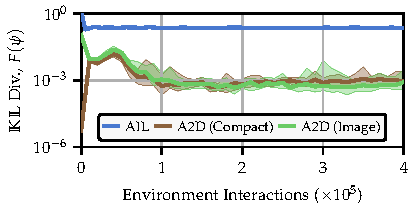
\includegraphics[width=0.95\textwidth]{figures/sec4/cr/lg/sec4_divergence_IceLake_True_cr_logs_LavaGap_LavaGapCompiledRun_.pdf}
        \caption{Frozen Lake.}
        \label{fig:grid:a2dplot:lg}
    \end{subfigure}%
    %
    \hfill%
    %
    \begin{subfigure}[t]{0.48\textwidth}
        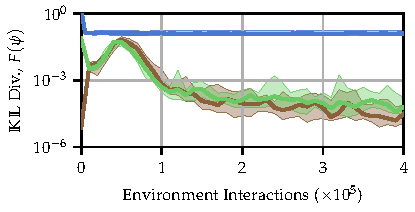
\includegraphics[width=0.95\textwidth]{figures/sec4/cr/td/sec4_divergence_TigerDoor_True_cr_logs_TigerDoor_TigerDoorCompiledRun_.pdf}
        \caption{Tiger Door.}
        \label{fig:grid:a2dplot:td}
    \end{subfigure}%
    \vspace{-0.2cm}
    \caption{The evolution of the policy divergence, $F(\psi)$.  Shown are median and quartiles across $20$ random seeds.  \emph{AIL} converges to a high divergence, whereas A2D achieves a low divergence for both representations, indicating that the trainee recovered by A2D is faithfully imitating the expert (see Figure \ref{fig:gridworld_asym} for more information). 
    { }%
    }
    \label{fig:grid:a2dplot}
\end{figure*}

